\documentclass[
  letterpaper,
  twocolumn,
  9pt,
  journal,
  final]{IEEEtran}

\usepackage[spanish,es-tabla]{babel}
\usepackage[utf8]{inputenc}
\usepackage{amsfonts}
\usepackage{amsmath}
\usepackage{amssymb}
\usepackage{amsxtra}
\usepackage{mathrsfs}
\usepackage{array}
\usepackage{tikz}
\usepackage{cite}
\usepackage{varioref}
\usepackage{float}
\usepackage{color}
\usepackage{colortbl}
\usepackage{enumerate}
\usepackage{rotating}
\usepackage{subcaption}
\usepackage{hyperref}
\usepackage{listings}
\usepackage{lipsum}
%\usepackage{flushend}
\usepackage{graphicx}

\usepackage{xcolor}
\hypersetup{
    colorlinks,
    linkcolor={red!50!black},
    citecolor={blue!50!black},
    urlcolor={blue!80!black}
}



\title{Tarea 4 - Procesamiento Digital de Imágenes}
\author{\textbf{Autor:} Pablo Yáñez Santibáñez - pablo.yanez@uai.cl}
%\author{\IEEEauthorblockN{Pablo Yáñez S.} - pablo.yanez@uai.cl}

% Levels to show in table of contents:
% \setcounter{tocdepth}{-1} % only parts
% \setcounter{tocdepth}{0}  % only parts and chapters
\setcounter{tocdepth}{1}  % part,chapters,sections
% \setcounter{tocdepth}{2}  % part,chapters,sections, subsections
% \setcounter{tocdepth}{3}  % part,chapters,sections, subsections,subsubsections
% \setcounter{tocdepth}{4}  % part,chapters,sections, subsections,subsubsections and paragraphs
% \setcounter{tocdepth}{5}  % part,chapters,sections, subsections, subsubsections, paragraphs and subparagraphs.


\begin{document}
\bstctlcite{IEEEexample:BSTcontrol}
\maketitle

% \begin{abstract}
% We propose \lipsum[1]
% \end{abstract}

\tableofcontents

% \listoffigures

% \listoftables

%%%%%%%%%%%%%%%%%%%%%%%%%%%%%%%%%%%%%%%%%%%%%%%%%%%%%%%%%%%%%%%%%%%%%%%%%%%%%%%%

\section{Introducción}

Para el desarrollo de este trabajo se descarga una imagen de Los Dientes de Navarino (Puerto Williams) del sitio \href{https://www.flickr.com/photos/whitewizard/7062826349/in/album-72157629780861323/}{Flickr}. Esta imagen es usada para las distintas actividades que se describen en este documento.

\begin{figure}[h!]
	\centering
	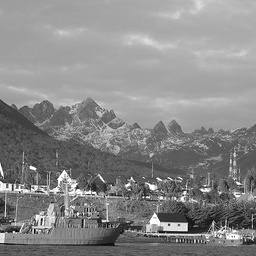
\includegraphics[width=0.7\linewidth]{outs/gaussiano/img.jpg}
	\caption{Dientes de Navarino.}
	\label{fig:dientes}
\end{figure}


\section{Marco Teórico}

\section{Ruido Gaussiano}

\section{Ruido Impulsional - Pimienta}

\section{Ruido Impulsional - Sal}

\section{Ruido Uniforme}


%%%%%%%%%%%%%%%%%%%%%%%%%%%%%%%%%%%%%%%%%%%%%%%%%%%%%%%%%%%%%%%%%%%%%%%%%%%%%%%%
% Bibliography
\nocite{*}
\bibliographystyle{IEEEtran}
\bibliography{bibliography}


\end{document}


% Photo:
% https://www.flickr.com/photos/carlosyanez/29061122837/



%\begin{lstlisting}[language=bash]
%  $ wget http://tex.stackexchange.com
%\end{lstlisting}

%\begin{table} \caption{A Simple Example Table} \label{table_example}
%  \begin{center}
%    \begin{tabular}{c c}
%      \hline
%      \bfseries First & \bfseries Next\\ \hline\hline
%      1.0 & 2.0 \\
%      \hline
%    \end{tabular}
%  \end{center}
%\end{table}


%\begin{lstlisting}[float=tbh!, caption={Magnitud de la respuesta en frecuencia del filtro IIR},label={cod:mag resp frec %IIR}]
%mag=20*log10(abs(H));
%\end{lstlisting}